\documentclass[10pt]{article}
\usepackage[a4paper, total={170mm, 257mm}]{geometry}

\usepackage[
backend=biber,
style=nature,
sorting=none
]{biblatex}
\addbibresource{References.bib}
%\bibliographystyle{unsrt}


\usepackage{amsmath}
\usepackage{amssymb}
\usepackage{upgreek}
\usepackage{dsfont}
\usepackage{esint} % various fancy integral symbols
\usepackage{mathrsfs} % for \mathscr

% fancy notation stuff
\usepackage{accents}
% vector arrows under the symbol to distinguish covariant and contravariant
\newcommand\undervec[1]{\underaccent{\vec}{#1}}

\usepackage{siunitx}
\DeclareSIUnit{\litre}{l} % litres as lower case l (upper case L by default)

%\usepackage{hyperref}

\usepackage{graphicx} % Required for inserting images
\usepackage{multicol}
\usepackage{mathpazo}
\usepackage[font=sf,labelfont=bf]{caption}

% title, headings, abstract heading in sans serif font and maybe color
%\usepackage{sectsty}
%\usepackage{titling}
%\usepackage[sf,bf,pagestyles]{titlesec}
\usepackage[dvipsnames]{xcolor}
\usepackage{sectsty}
\usepackage{abstract}
\renewcommand\abstractnamefont{\sffamily\bfseries}%\color{Maroon}}
%\chapterfont{\color{blue}}  % sets colour of chapters
\sectionfont{\sffamily}%\color{Maroon}}  % sets colour of sections
\subsectionfont{\sffamily}%\color{Maroon}}  % sets colour of subsections
\subsubsectionfont{\sffamily}  % sets colour of subsections





% TO DO's
\newcommand{\todo}[1]{ {\color{ForestGreen} [#1]} }

\graphicspath{{figures/}}

\usepackage{lipsum} 

% referencing commands
\newcommand{\seefig}[2]{\mbox{\sffamily($\rightarrow$ Fig. \ref{#1}#2)}}
\newcommand{\reffig}[2]{\mbox{\sffamily{Figure \ref{#1}#2}}}


\title{\sffamily\bfseries\color{MidnightBlue} Scattering Spectroscopy of\\Plasmonic Janus Particles\\\mbox{ }\\Supplementary Material}
\author{Felix H. Patzschke, A. Markus Anton and *Frank Cichos}
%\date{November 2023}
\date{}



\begin{document}
%\allsectionsfont{\sffamily}

\maketitle

\sectionfont{\sffamily\color{MidnightBlue}}  % sets colour of sections
\subsectionfont{\sffamily\color{MidnightBlue}}  % sets colour of subsections



\section*{Derivation of the probability density for the out-of-plane angle}

The model JP is cylindrically symmetric. Therefore its orientation in space is completely described by the direction of its axis of symmetry, $\hat{z}$. 
For the random orientation, let $\hat{z}$ be evenly distributed over $\mathcal{S}^2$. 
For a PDF $p_\Omega$ w.r.t. the solid angle $\Omega$, this means
$$
\iint_{\mathcal{T}} p_\Omega \ \mathrm{d}\Omega
=
\frac{
\iint_{\mathcal{T}} \mathrm{d}\Omega
}{
\varoiint_{\mathcal{S}^2} \mathrm{d}\Omega
}
\quad\forall\ \mathcal{T}\subseteq\mathcal{S}^2
\ .
$$
$\varoiint_{\mathcal{S}^2} \mathrm{d}\Omega$ is nothing else than the surface area of the unit sphere, $4\pi$. 
Therefore, 
$$
\iint_{\mathcal{T}} p_\Omega \ \mathrm{d}\Omega
=
\frac{1}{4\pi}\ 
\iint_{\mathcal{T}} \mathrm{d}\Omega
\quad\forall\ \mathcal{T}\subseteq\mathcal{S}^2
\ ,
$$
which implies that
$$
p_\Omega=\frac{1}{4\pi}\ .
$$

Now, we parametrise $\mathcal{S}^2$ in spherical coordinates $(\alpha,\beta)$, where $\alpha$ is the polar coordinate and $\beta$ is the azimuthal coordinate. 
The differential solid angle is
$$
\mathrm{d}\Omega = \sin\alpha \ \mathrm{d}\alpha \ \mathrm{d}\beta \ .
$$
The PDFs w.r.t. these coordinates, $p_{\alpha}$ and $p_\beta$, must satisfy
$$
\begin{aligned}
\text{a)}&&
\int_0^\pi p_{\alpha} \ \mathrm{d}\alpha &= 1
\\
\text{b)}&&
\int_0^{2\pi} p_{\beta} \ \mathrm{d}\beta &= 1
\\
\text{and c)}&&
\iint_{\mathcal{T}} p_\alpha \cdot p_\beta \ \mathrm{d}\alpha\ \mathrm{d}\beta
&=
\iint_{\mathcal{T}} p_\Omega \ \mathrm{d}\Omega
\quad\forall\ \mathcal{T}\subseteq\mathcal{S}^2
\ .
\end{aligned}
$$
From \mbox{c)}, it follows that
$$
\begin{aligned}
p_\alpha \cdot p_\beta \ \mathrm{d}\alpha\ \mathrm{d}\beta &= p_\Omega \ \mathrm{d}\Omega
\\
&= \frac{1}{4\pi} \ \sin\alpha \ \mathrm{d}\alpha \ \mathrm{d}\beta \ .
\end{aligned}
$$
Cancelling $\mathrm{d}\alpha\ \mathrm{d}\beta$ yields
$$
p_\alpha \cdot p_\beta = \frac{1}{4\pi} \ \sin\alpha \ .
$$
To separate $p_\alpha$ and $p_\beta$, let's assume that $p_\alpha$ and $p_\beta$ are invariant w.r.t. $\beta$ and $\alpha$, respectively. 
Then, substitution in \mbox{a)} yields
$$
\begin{aligned}
\frac{1}{p_\beta} \int_0^\pi p_\alpha \cdot p_\beta \ \mathrm{d}\alpha &= 1
\\
\frac{1}{4\pi\ p_\beta} \underbrace{\int_0^\pi \sin\alpha \ \mathrm{d}\alpha}_{=2} &= 1
\quad\therefore\quad
p_\beta = \frac{1}{2\pi}
\ ,
\end{aligned}
$$
which also satisfies \mbox{b)}. 
It follows that 
$$p_\alpha = \frac{\sin\alpha}{2} \ .$$



\section*{Integration of the Far-Field Intensities}

For a given incident wavelength and illumination angle, let the scattering intensity in the far-field be
$$I_\mathrm{far}(\theta,\phi)\ .$$
The data retrieved from the simulation are $I_n$, samples of $I_\mathrm{far}$ in points $\left( \theta_n, \phi_n \right)$ on the unit sphere $\mathcal{S}^2$. 
To compute
$$
    \iint_{\mathcal{T}} I_\mathrm{far} \ \mathrm{d}\Omega \approx \sum_{n \vert \left( \theta_n, \phi_n \right)\in\mathcal{T}} I_n \ \Delta\Omega_n \ , 
$$
we must determine the values of $\Delta\Omega_n$. [TODO: Notation]

We project the spherical coordinates $\left( \theta_n, \phi_n \right)$ into the Euclidean plane, obtaining the cartesian coordinates $(x_n, y_n)$.\footnote{The choice of projection is somewhat arbitrary, we chose the stereographic projection.} 
We then compute the Voronoi tesselation which maps each projected sample point $(x_n, y_n)$ to an area element\footnote{the fact of which being a convex polygon being computationally convenient, yet analytically irrelevant} 
$$
P_n = \left\lbrace 
(x,y) \in \mathds{R}^2 
\middle\vert 
\mathrm{arg}\min\limits_{n'} \Bigl( m_\mathrm{E}\bigl( (x,y)-(x_{n'},y_{n'}) \bigr) \Bigr)
= n
\right\rbrace
$$ 
with the Euclidean metric $m_\mathrm{E}$. 
The area elements $\Delta\Omega_n$ are then given as 
$$
\Delta\Omega_n
=
\mu\left(
P_n \cap \mathcal{T}
\right) \cdot \tau\left( \theta_n, \phi_n \right)
$$
where $\mu(\cdot)$ denotes the measure of a subset of $\mathds{R}^2$ and $\tau$ is the area element transfer function associated with the chosen projection. 









\section*{More Angular Distributions}

\begin{figure*}[b!]
    \centering
    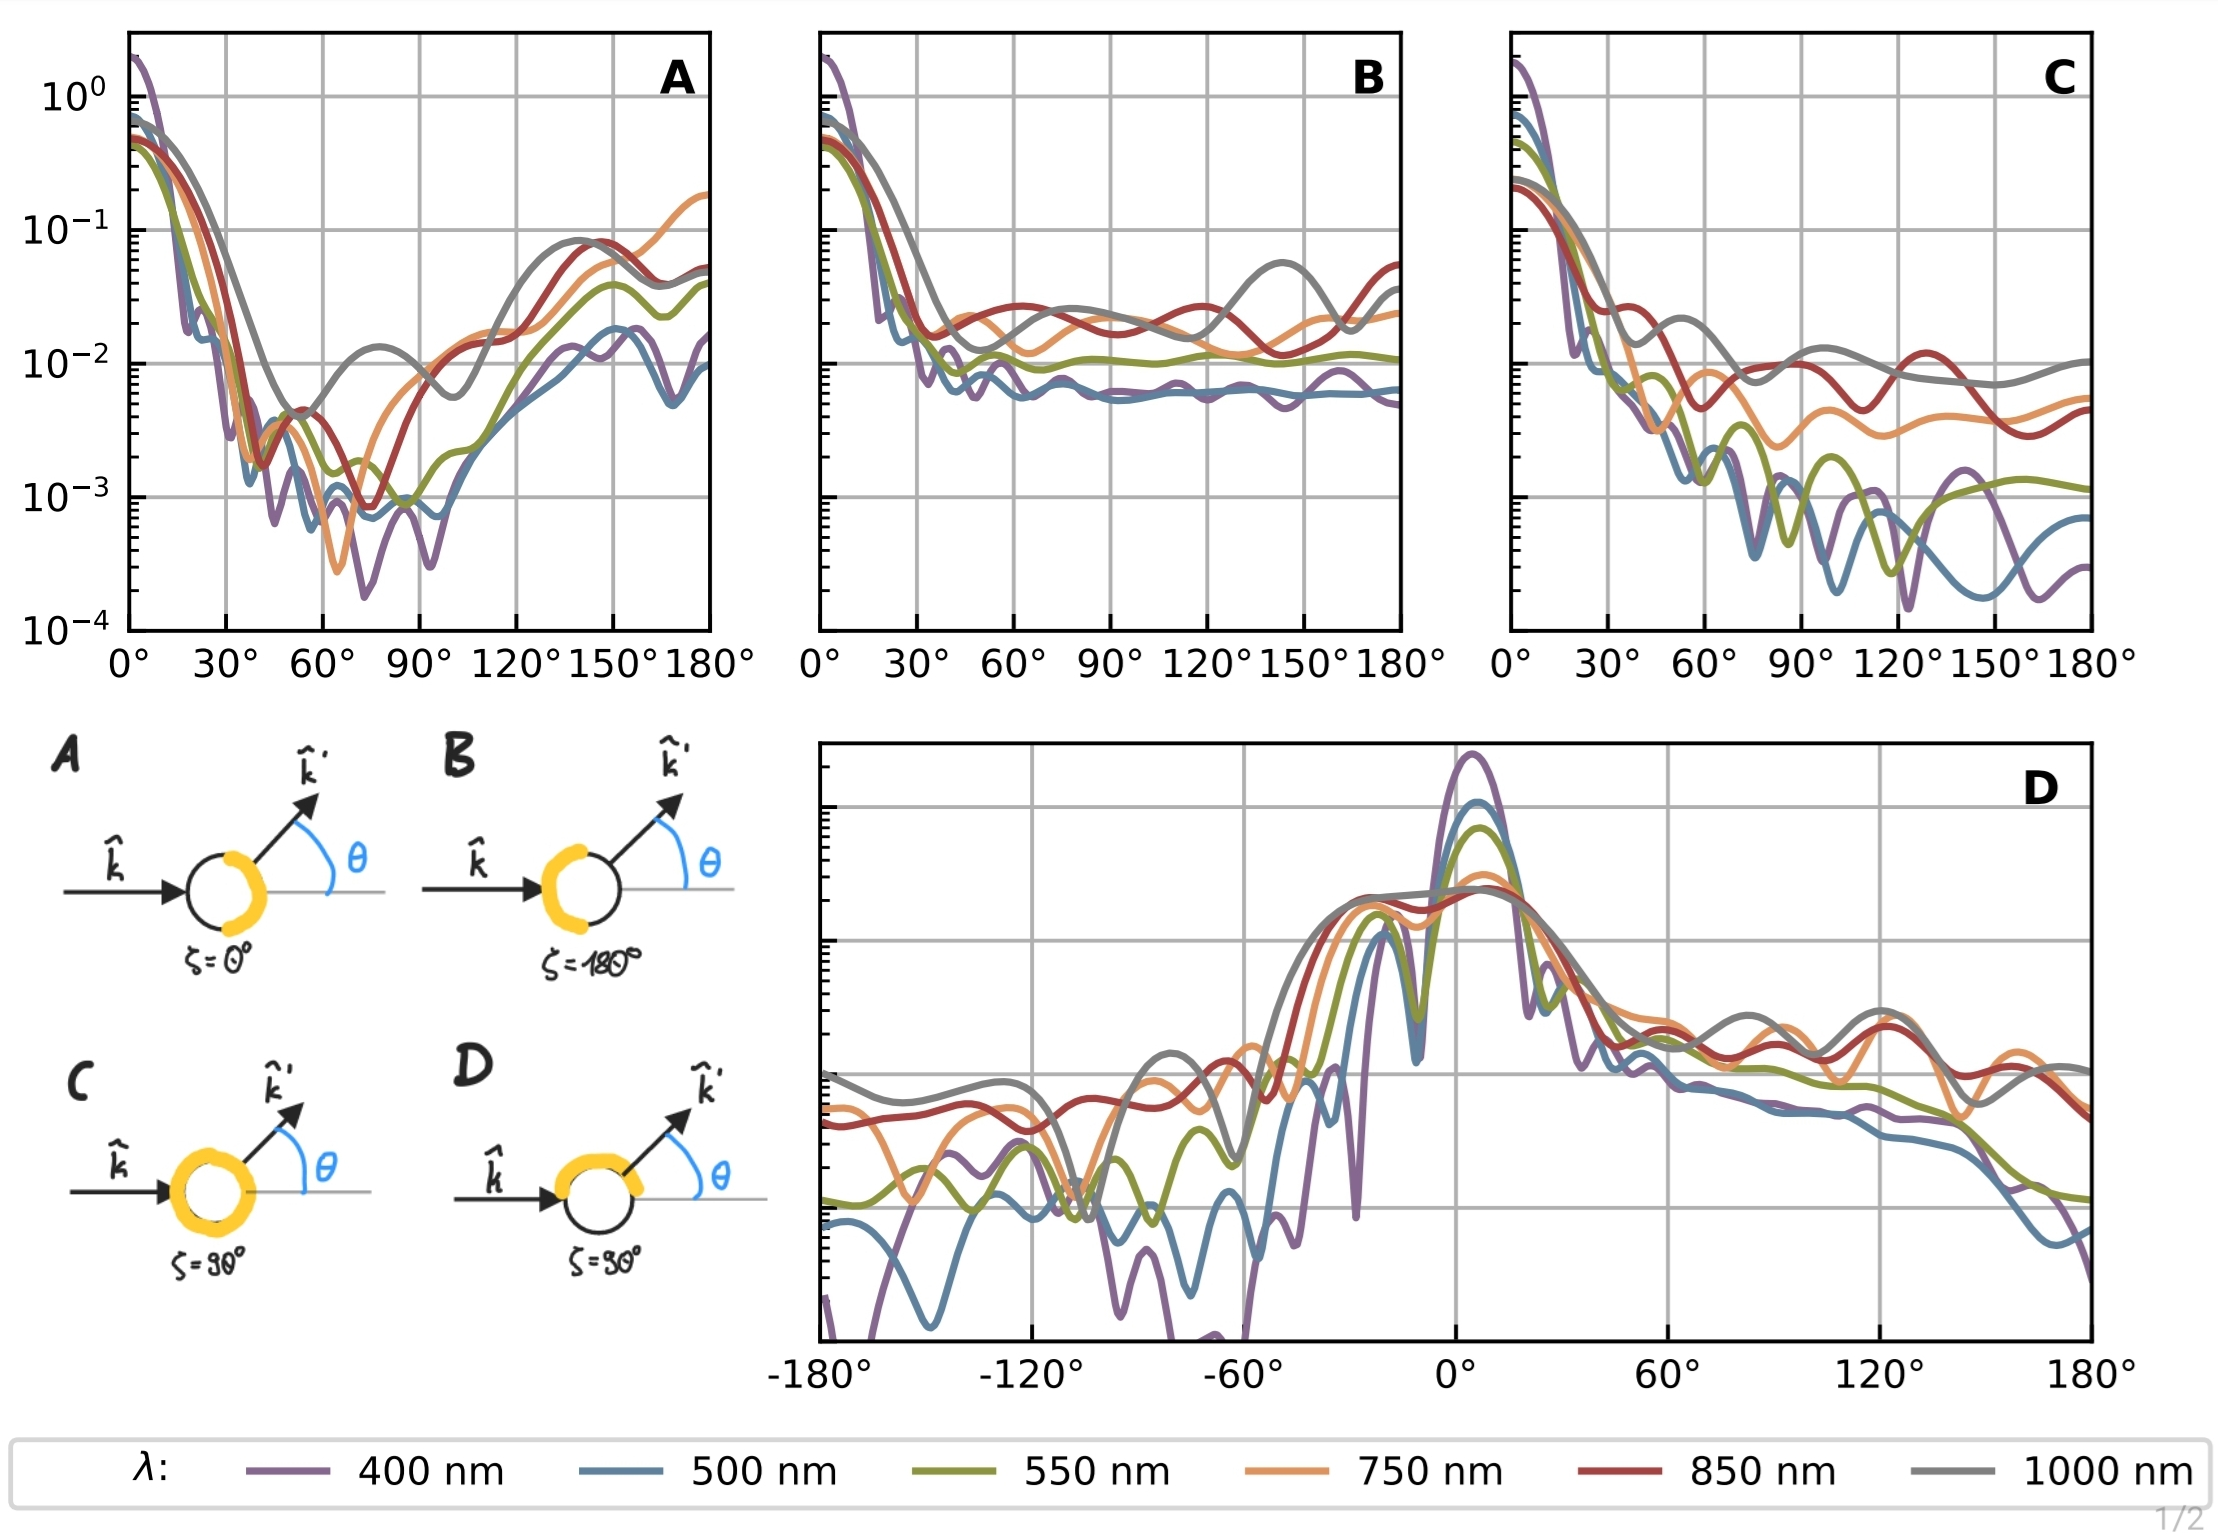
\includegraphics[width=\textwidth]{[fig] cartesian mieplots (placeholder).jpg}
    \caption{Scattering intensity of the JP versus scattering angle. 
    {\sffamily\bfseries A} and {\sffamily\bfseries B} show the cylindrically symmetric cases of illumination from the PS side and from the Au side, respectively, i.e. where $\hat{k}\parallel\hat{z}$. 
    In {\sffamily\bfseries C} and {\sffamily\bfseries D}, the light is incident side-on ($\hat{k}\perp\hat{z}$, $\zeta=\pi/2$).
    The scattering intensities are taken from the $(\hat{k},\hat{y})$ plane in {\sffamily\bfseries C} (note, that the system is still symmetric under inversion of $y$) and from the $(\hat{k},\hat{z})$ plane, where spatial symmetry is entirely broken, in {\sffamily\bfseries D}.
    Here, the Au side lies in the positive $\theta$ direction.  
    }
    \label{fig:jp-mieplots}
\end{figure*}


\end{document}
